\chapter{Future Work}
\label{ch:future}


\section{Vision of a WPT System using TR}
\label{sec:future-roadmap}
This research represents a first step in the exploration of building a
time reversal WPT system.
%
We demonstrate one possible realization of this idea in Fig.~\ref{fig:SysImage}.


The proposed system consists of two basic components.
%
The first is a rectenna that serves as the receiver.
%
The system as described in Section~\ref{sec:ltr-meth} would require an
out-of-band feedback channel between the receiver and transmitter. However, we
have demonstrated in Section~\ref{sec:selective-sim} that a transmitter can target
receivers entirely in-band.
%
Our system in Fig.~\ref{fig:SysImage} builds on these findings.
%
The second is a transmitter that performs the time reversal process.
%
This component is responsible for recording characteristic signals from the
receiver(s), time reversing the signals, and re-broadcasting them into the
environment.



In a practical system, the rectenna will be integrated into the hardware of a
mobile device, or into an external component that plugs into the battery.
%
The transmitter would  be connected to an external power source, but
could otherwise be located anywhere in the room.

Although not a component of the system, another important consideration in this
scenario is the environment; a low-loss scattering environment is necessary for
time reversal to be effective.

\begin{figure}[t]
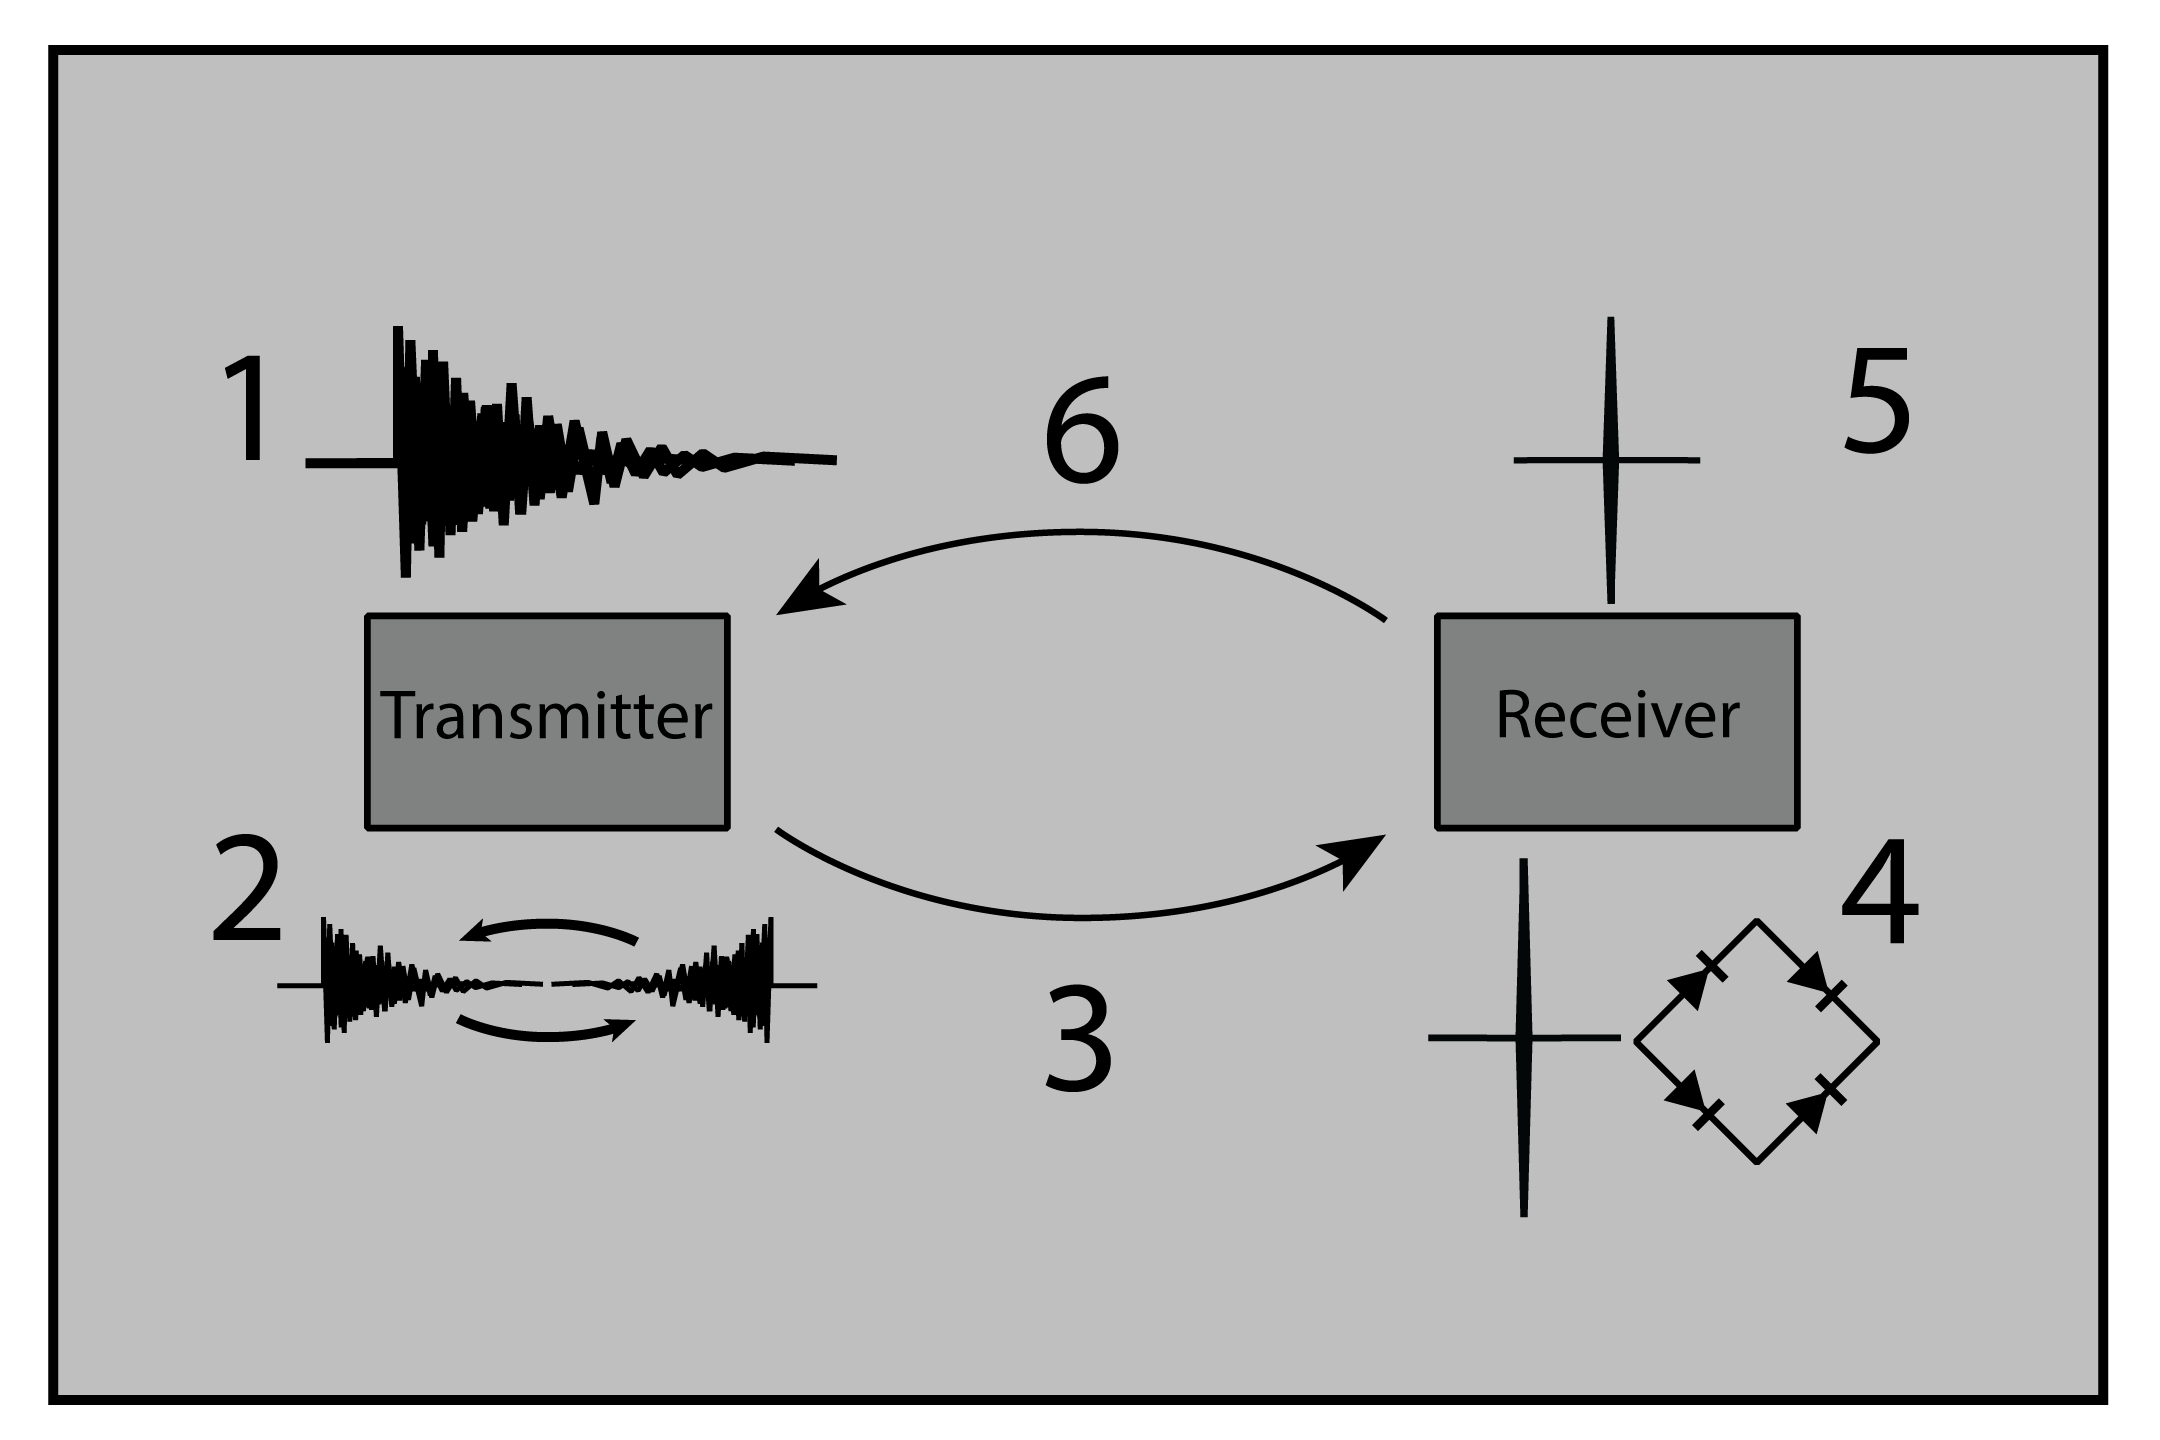
\includegraphics[width=\columnwidth]{figs/future/WPTSys}
\caption[Proposed Time Reversal System]{A notional time reversal WPT system. In the acquistion phase, a new receiver joins the system by broadcasting or emitting a characteristic signal (0). Here, the receiver actively emits a signal, but it is also possible for the transmitter to find a passive target, as shown in~\cite{nltr-wave-chaotic}. In either case, the next sona that the transmitter collects will contain spatial information unique to the receiver's location (1). In the power transfer cycle, the sona is time reversed (2), amplified, and broadcast back into the environment. The amplified signal reconstructs on the receiver (3) and is converted to usable DC power by the rectifier (4). A small fraction of the signal is used to re-broadcast a new characteristic signal (5) into the environment, which will be collected in the next sona (6). The cycle repeats from (2).}
\label{fig:SysImage}
\end{figure}

We have demonstrated the underlying concepts of the WPT system depicted in Fig.~\ref{fig:SysImage}.
However, much work is necessary to transform this proof-of-concept technology to a functional product that consumers may use.
Future work discussed here falls into one of two categories. The first category includes established TR techniques that may be extended into the field of TR WPT.
The second category includes novel designs proposed by the team applicable only to TR WPT. Both will be discussed below. 

\section{Future work on applying other techniques from TR to WPT}
\label{sec:future-tr}
Imaging of objects and non-invasive surgery are already common applications of TR.
As a result, many techniques have been developed to improve reconstruction quality on a target.
We suspect that many of these techniques may have applicability to our proposed system, but did not
have the opportunity to investigate them in our research.
However, stationary TR methods have different design priorities than our proposed TR WPT system.
Some modifications on the basic TR methodology that has been developed for these purposes may prove useful for an application to WPT. We suggest that future research be dedicated to investigating the applicability of techniques such as iterative time reversal and super-resolution to a practical WPT scheme.

\subsection{Iterations}

It has been well proven in the literature that time reversal focusing on an object can be repeated to improve waveform collapse on a target. ~\cite{prada_iterative_1991} However, this technique has not yet been applied to TR WPT.

We suspect that applying iterative TR to reduce the effect of reflection orbits which contribute poorly to the final reconstruction, in favor of ones that do. The side lobes in the time domain are representative of energy that may not be able to be rectified unless they are combined into the main peak. We predict that we can maximize our efficiency and reconstruction quality using this method. Additionally, we predict that this method will only be useful for stationary targets. Because iterating the time reversal process takes several more steps, the length of time required to focus on a target is increased considerably. Since the technique for focusing upon a moving receiver proposed earlier relies upon repeating the time reversal process many times, it may not be acceptable for the time required to perform TR to increase several hundred percent. 

Both of these characteristics can be easily tested, using algorithms already applied to acoustic TR. An experimental setup very similar to ours could be applied to this research. A faster sona refresh rate would be required from the TR system for this method to be able to outpace the natural ``decay'' of the testing environment. Once an iterative algorithm has been tested and found successful it should be tested in a less homogeneously reflective environment, to determine if it can be used to improve efficiency in lossy environments.

The novelty of such research is primarily in the characteristics measured. The demonstration (or lack thereof) of filtering of lossy paths would also be a major finding. Models should be generated relating the sona refresh rate to performance gains using iterative method. If possible, multiple environments should be tested to generalize these results.

\subsection{Multiple Transmitters}

Many TR applications make use of multiple transmitters as a method of improving signal quality. Time reversal with multiple transmitters has the effect of improving the reconstruction strength at a target point, because more paths can be utilized to increase the superposition of the reconstruction pulses. All research done by the team was performed using a single transmitting antenna. The incorporation of multiple antennas would require major modifications to our experimental setup, and was beyond our capabilities at this time.

While final signal strength of the reconstruction is predicted to increase, how much remains to be determined. Future research should attempt to determine how the use of multiple antennas relates to the efficiency of energy transfer. Particular attention should be paid to how this efficiency changes as sources of loss are introduced into the system.

\subsection{Exponential Amplification}

From \cite{Biniyam} we know that exponential amplification can be used to counteract decreased reconstruction quality caused by system losses. Exponential sona amplification is a nonlinear amplification to the sona across its timespan. It is meant to counteract the larger losses (due to larger number of reflections) experienced by reflective orbits with larger paths.

However, it should be understood that this method only compensates for the losses experienced by a time reversed signal. It does not avoid losses, and in fact more energy is lost through this method. As a result, efficiency using this method should decrease. This introduces a tradeoff to using the method that could be significant to designers of a TR WPT system. Quantifying the aspects of this tradeoff in a WPT context so that informed decisions can be made in the design of future systems.

\section{New problems that arise with TR in a WPT context}
\label{sec:future-wpt}

There are additional challenges involved with a TR WPT sytem that create avenues for research and innovation. Many of these deal with addressing the differing design goals with a TR WPT system - most TR applications care little about efficiency, caring only about the fidelity of the reconstruction on the target. In TR WPT the opposite is true - perfect reconstructions are far less important than the efficiency of transfer. Most TR applications consider stationary - or near stationary - targets. TR WPT system must always consider moving targets, or at least stationary targets within a dynamic environment.

These and other considerations set TR WPT apart from other TR research, and require the development of novel techniques. Below we suggest several TR WPT-specific research topics, experiments that could explore them, and how the results of these experiments can benefit TR WPT.

\subsection{Sub Cavity}

The demand for optimal efficiency requires TR WPT to consider the characteristics of the environment moreso than ordinary TR applications. It is clear to the team that a TR WPT system will likely need some environmental modifications to achieve an efficiency sufficient to see practical application. These modifications should also be designed to be as cheap and simple to install as possible, to ensure that system price remains practical.

We suggest that the easiest method to improve efficiency of TR wireless power transfer is to introduce a ``sub cavity'' within the transfer environment. This ``sub cavity'' will be defined as a region of the environment that allows extremely efficient TR WPT. The sub cavity becomes much less lossy than the environment as a whole. TR paths will preferentially move through the sub cavity, and can dramatically improve the efficiency of the entire system. A successful sub cavity must have the following characteristics:

\begin{itemize}
  \item High transfer efficiency/low reflective losses
  \item Chaotic geometry to facilitate the function of TR
  \item Presence of one or more paths between the sub cavity and main environment
\end{itemize}

There are many methods that could potentially generate such a cavity - a proposal for such as system can be found in Fig.~\ref{fig:subCav}. This cavity is a thin sheet of material that would be mounted to the ceiling of the room in question. The material in this sheet should have a smaller index of refraction than air; as a result any signal broadcast into can become ``trapped'' in the layer. At any given point along the barrier of the sub cavity only small amounts of signal will return to the main environment. A TR WPT system can selectively choose paths through the sub cavity that will focus on a given receiver with high transfer efficiency. Reflectors can be added to the sub cavity as needed to ensure that its complexity is enough to allow TR to occur.

\begin{figure}[h]
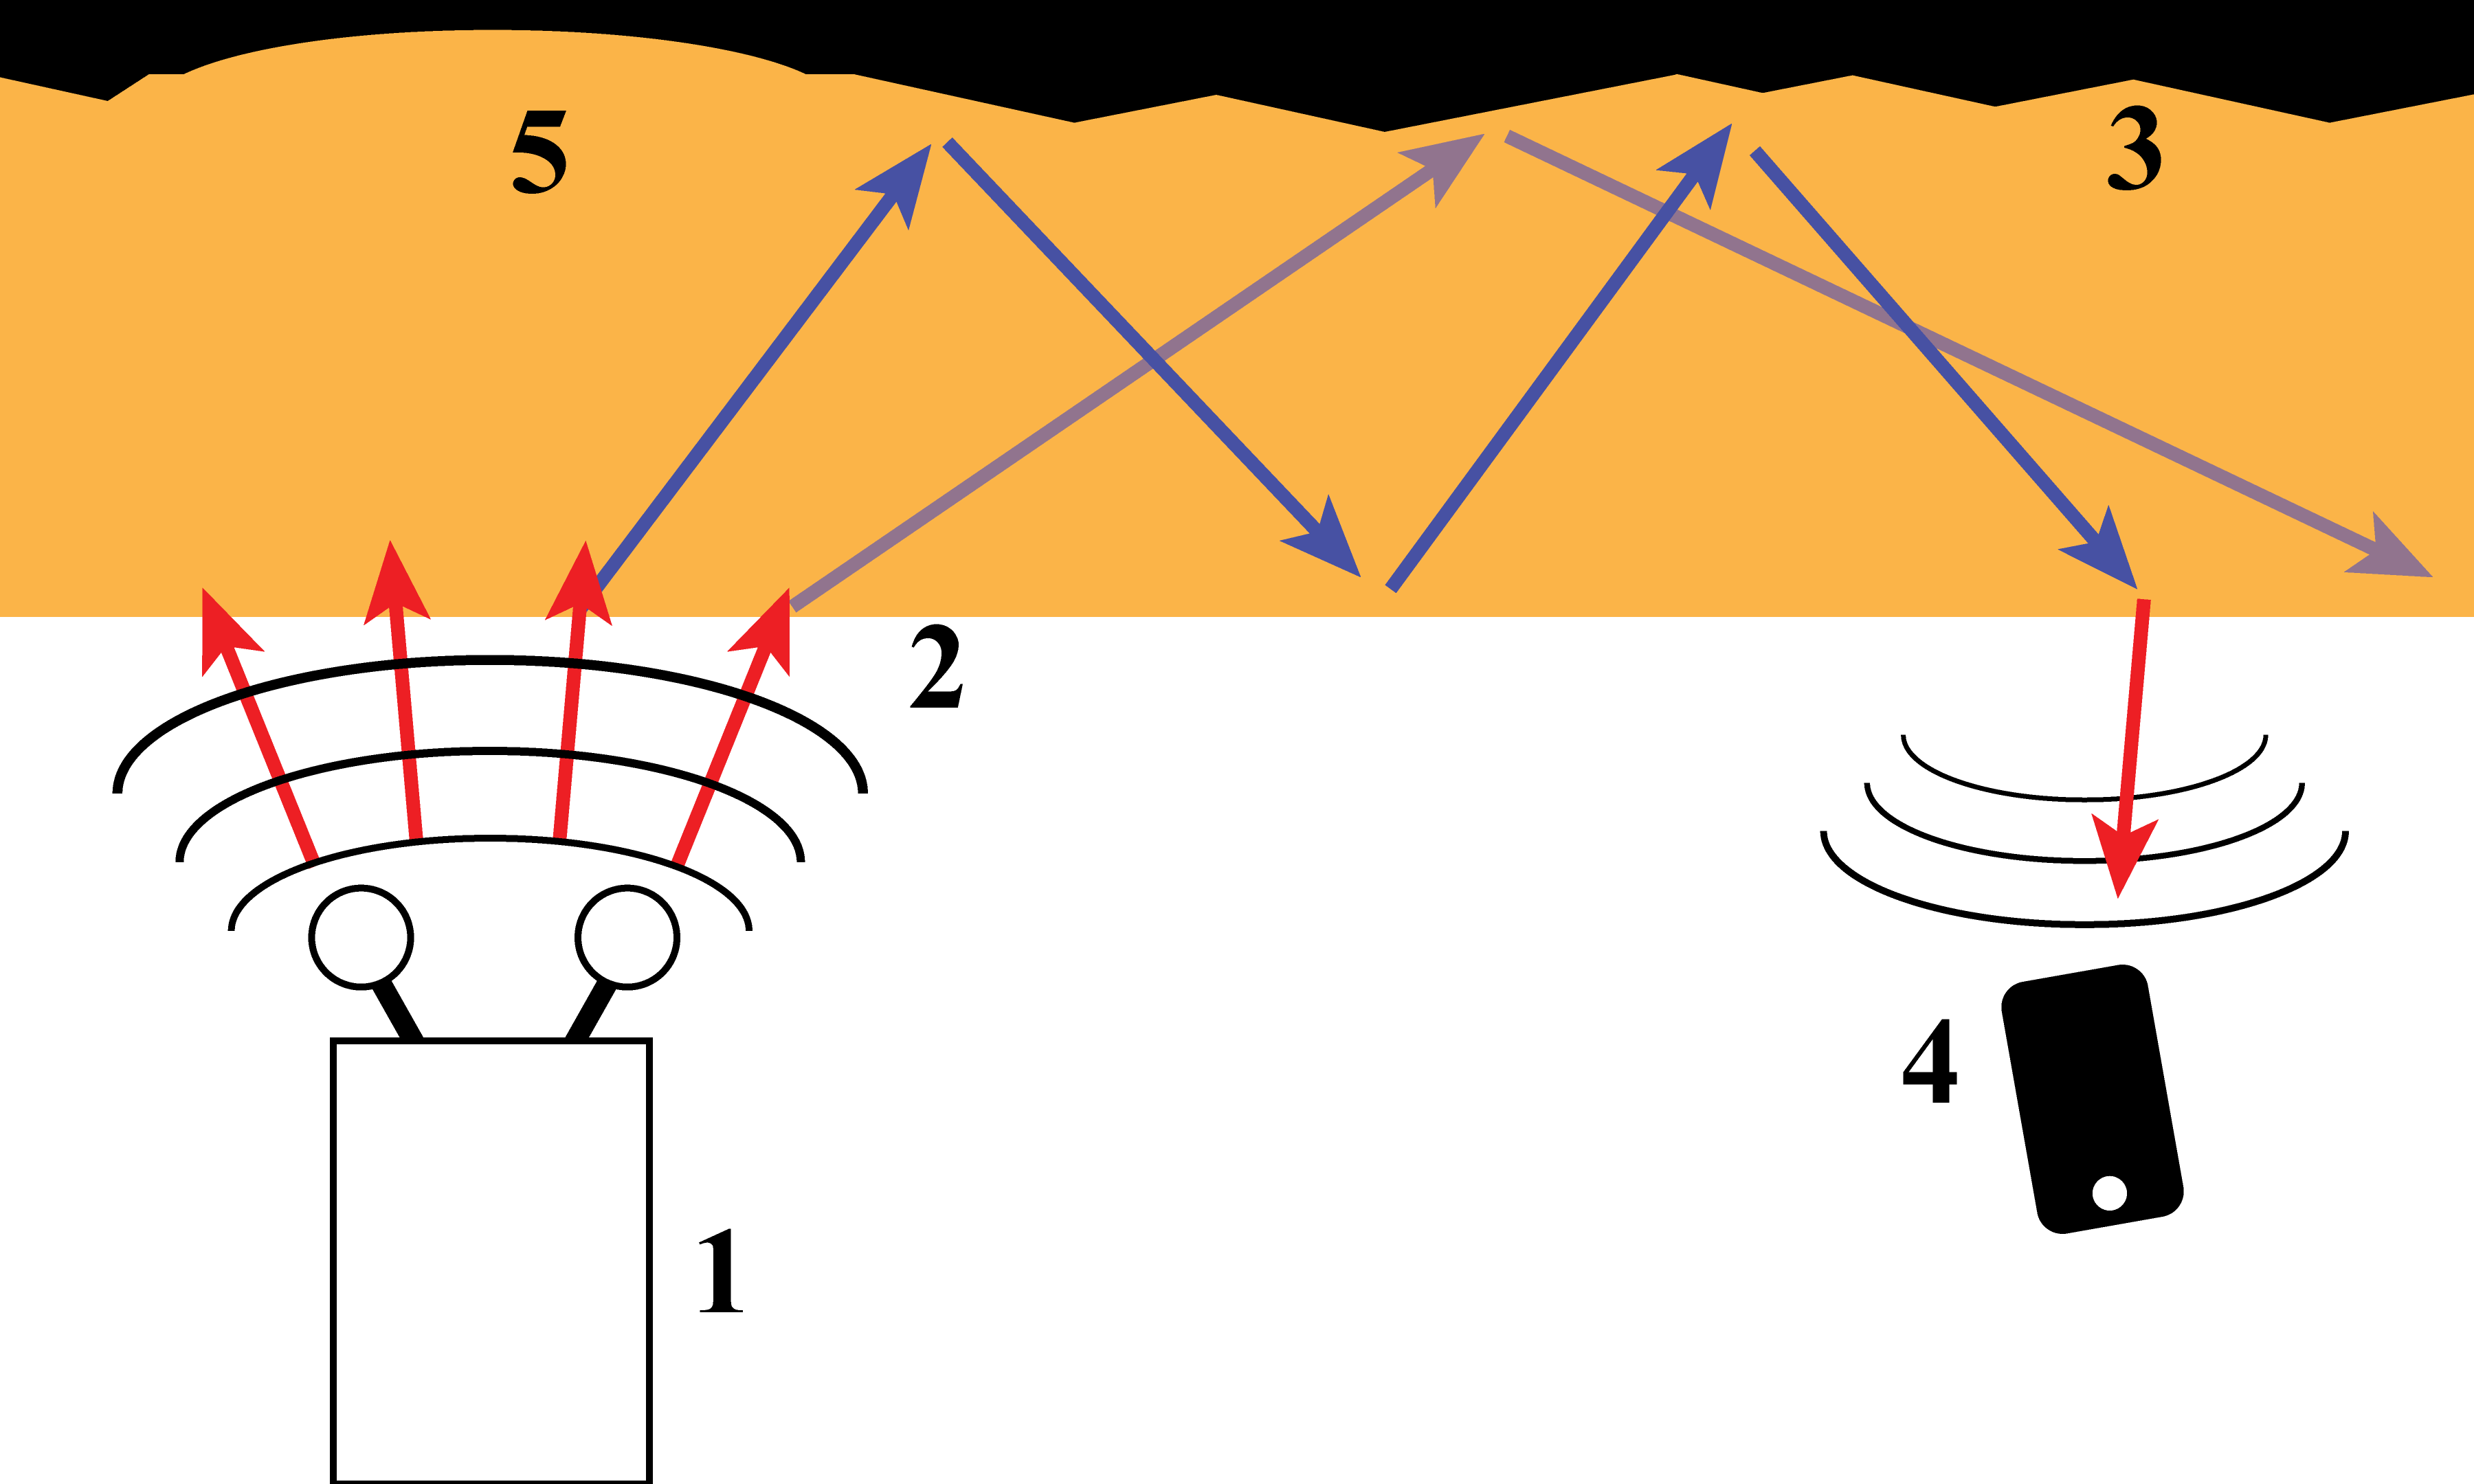
\includegraphics[width=\columnwidth]{future/subCavity}
\caption[Proposed ``Sub Cavity Design'']{A proposed sub cavity design. A transmitter (1) broadcasts an interrogation pulse into the environment. When the pulse reaches the low index of refraction material of the sub cavity, it refracts, taking on a lower angle (2). The interrogation pulse totally internally reflects within the cavity (3), until returning to the main environment. Some aspects of the signal reach the receiver, allowing a TR link to be established (4). A focal aspect of the geometry above the transmitter (5) is highlighted as a way of improving transmission.}
\label{fig:subCav}
\end{figure}

Research would focus on, firstly, proving that this method can work for the purposes of increasing efficiency of transfer. Once this has been established, the geometry of the sub cavity should be optimized to work in a wide range of potential environments. Uniformity of signal coverage is a major concern, and must be tested either experimentally, or through use of simulation software.

\subsection{Protection of Information}
Many of the improvements suggested above are focused on increasing the efficiency of the final system. Most of these improvements assume that while the system may be lossy, it is enclosed. That is, while signals may be absorbed by the environment, they are not lost completely. However, complete loss can be expected to occur often in practical applications. This can be due either due to holes in the environment (such as windows or doors) or heavily absorptive materials. The use of a selective transmission channel (as proposed above) may mitigate the effects of a channel through which a signal may escape. However, other methods should also be considered.

Earlier our concern with losses focused primarily on their impact on efficiency. Information transfer was sufficient to allow TR to occur. However, complete losses remove information from the system, and severely damage the ability for TR to reconstruct on a target. We believe that this can be visualized using the idea of loss of outgoing paths. Fig.~\ref{fig:outgo} shows how time reversal can be impacted by environments with complete loss.

\begin{figure}[h]
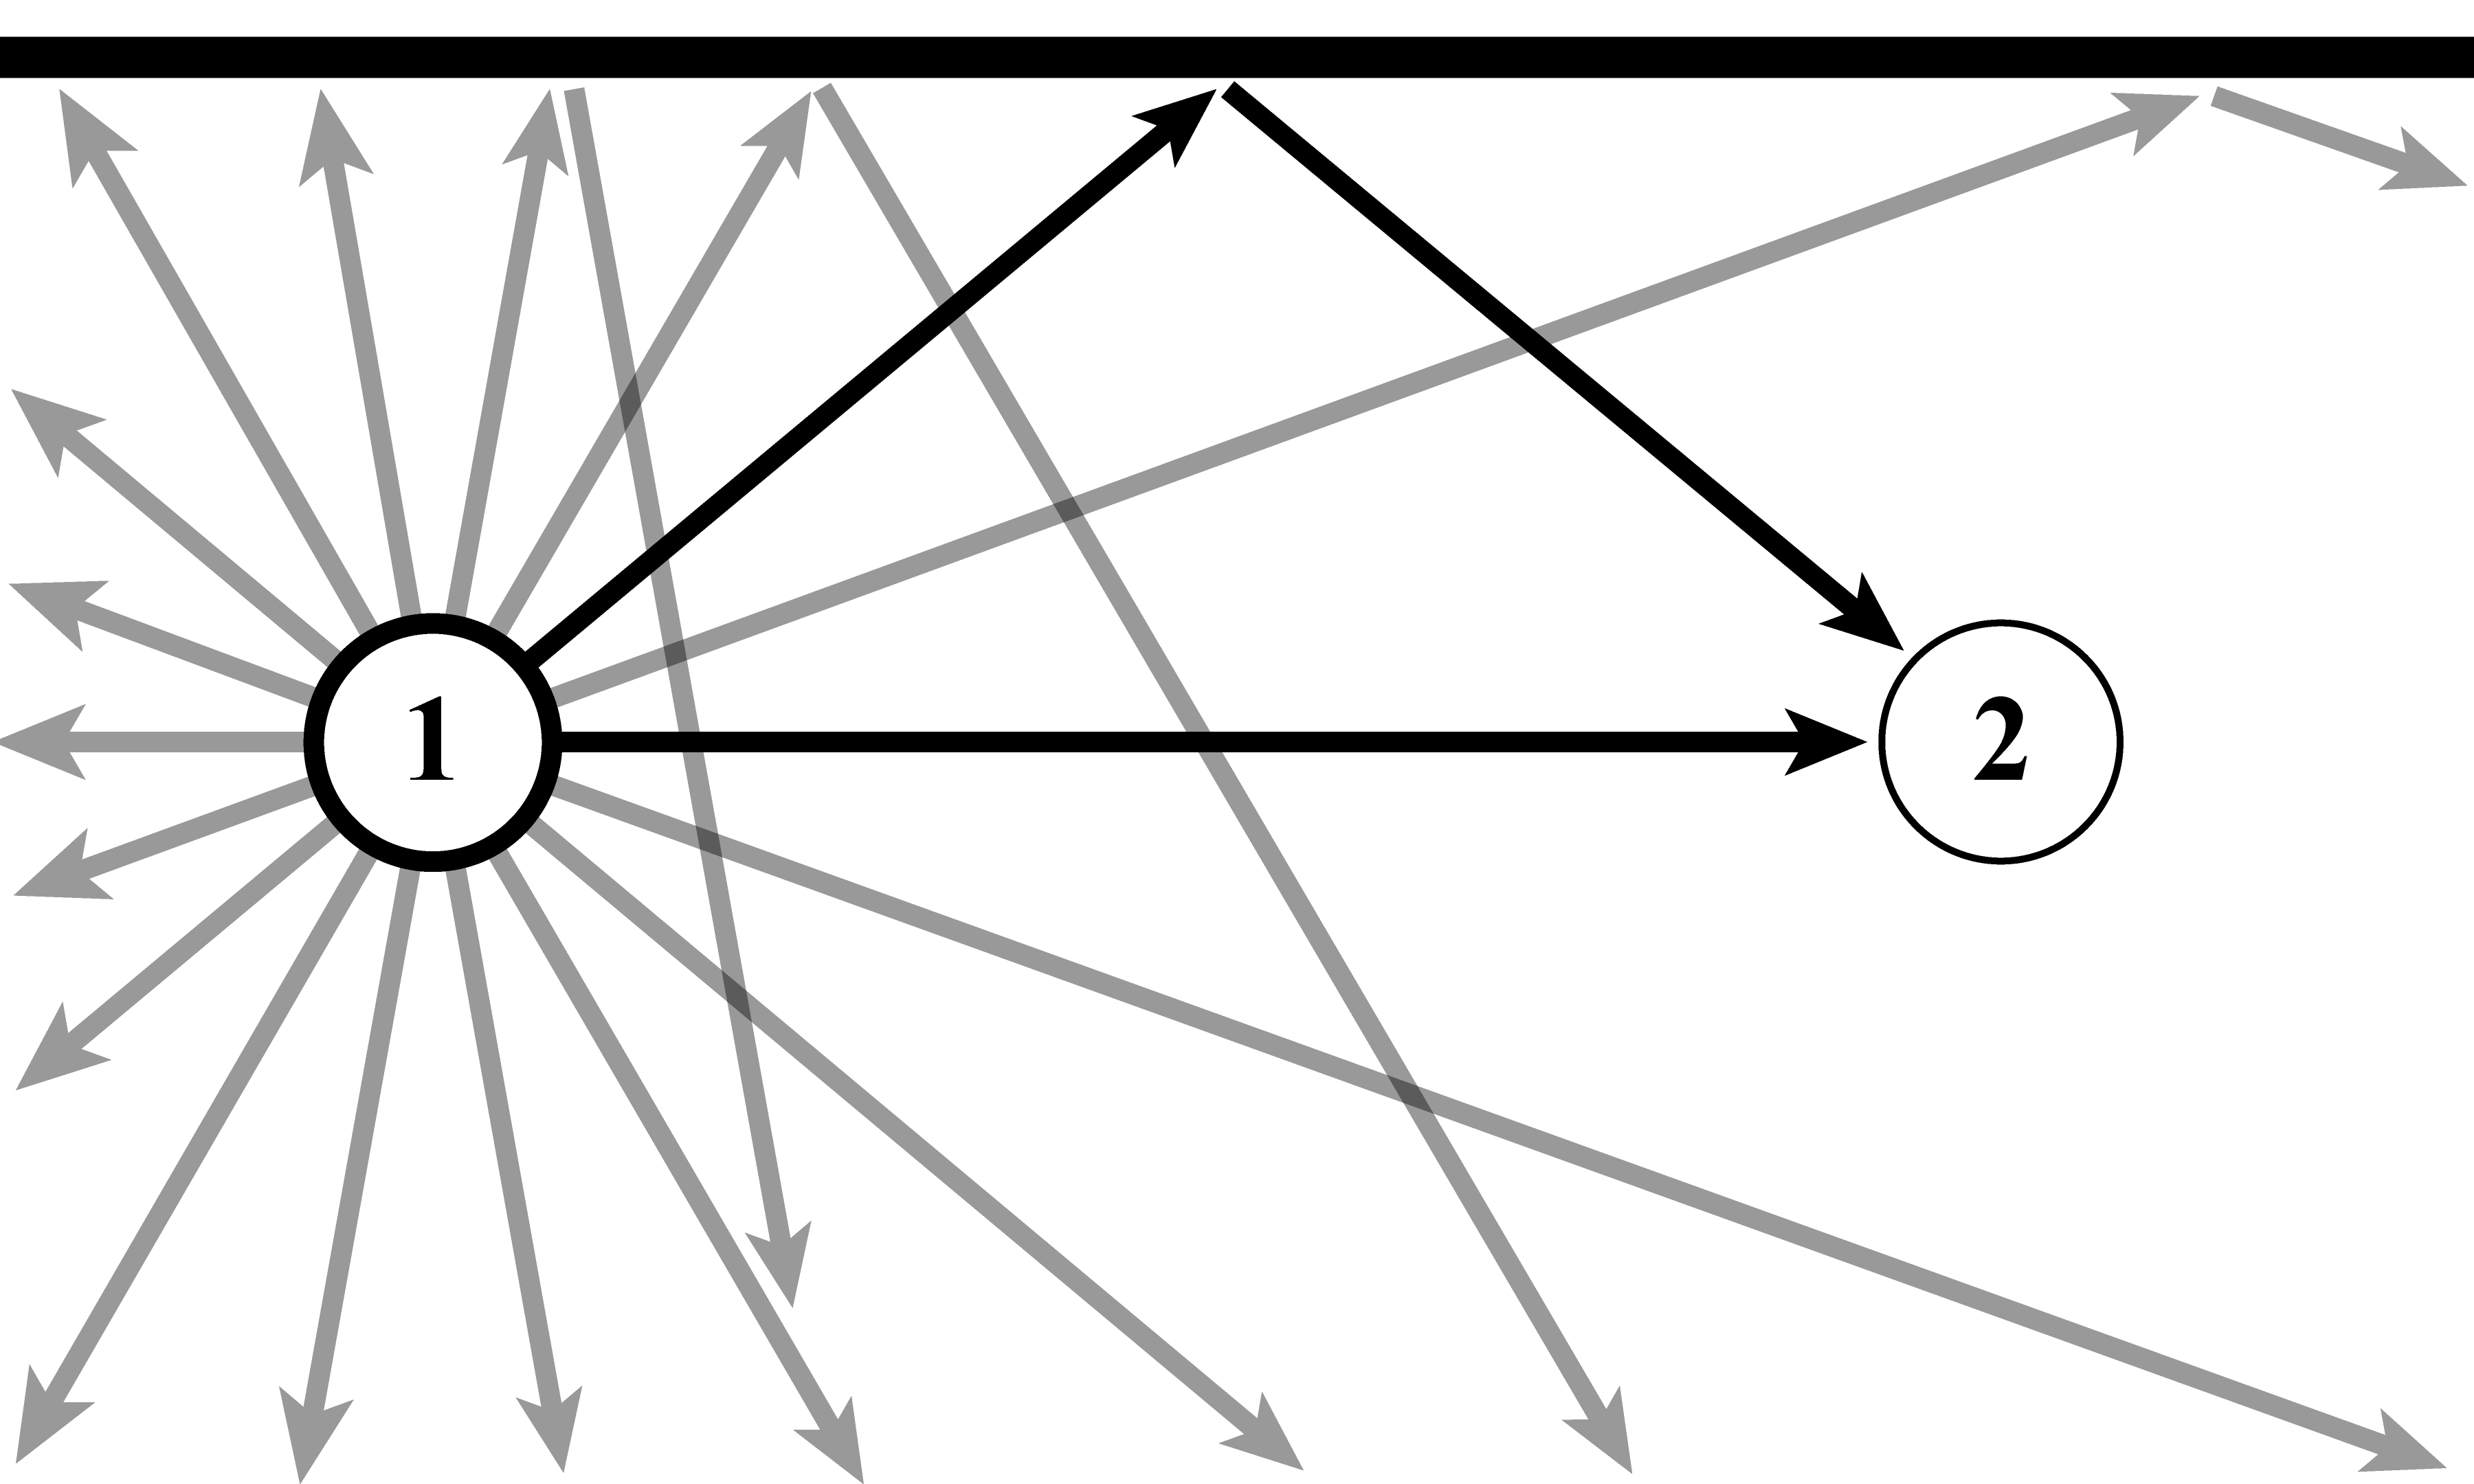
\includegraphics[width=\columnwidth]{future/outgoing}
\caption[Example of information loss on time reversal efficacy]{A representation of how complete losses affect time reversal. In this scenario, a transmitter (1) sends a signal in all directions in an environment with only one reflective surface. As can be seen, only a small percentage of the energy successfully reaches the receiver (2). If time reversal from (2) to (1) were to be attempted, a small and spatially unbalanced amount of energy would arrive at (1), resulting in a poor reconstruction.}
\label{fig:outgo}
\end{figure}

This is partly why a large number of reflective surfaces is beneficial in a time reversal environment. However, we believe that this effect is more advantageous (from an information protection point of view) when it occurs near to the target of the time reversal process. This concept is discussed in Fig.~\ref{fig:infoProtection}

\begin{figure}[h]
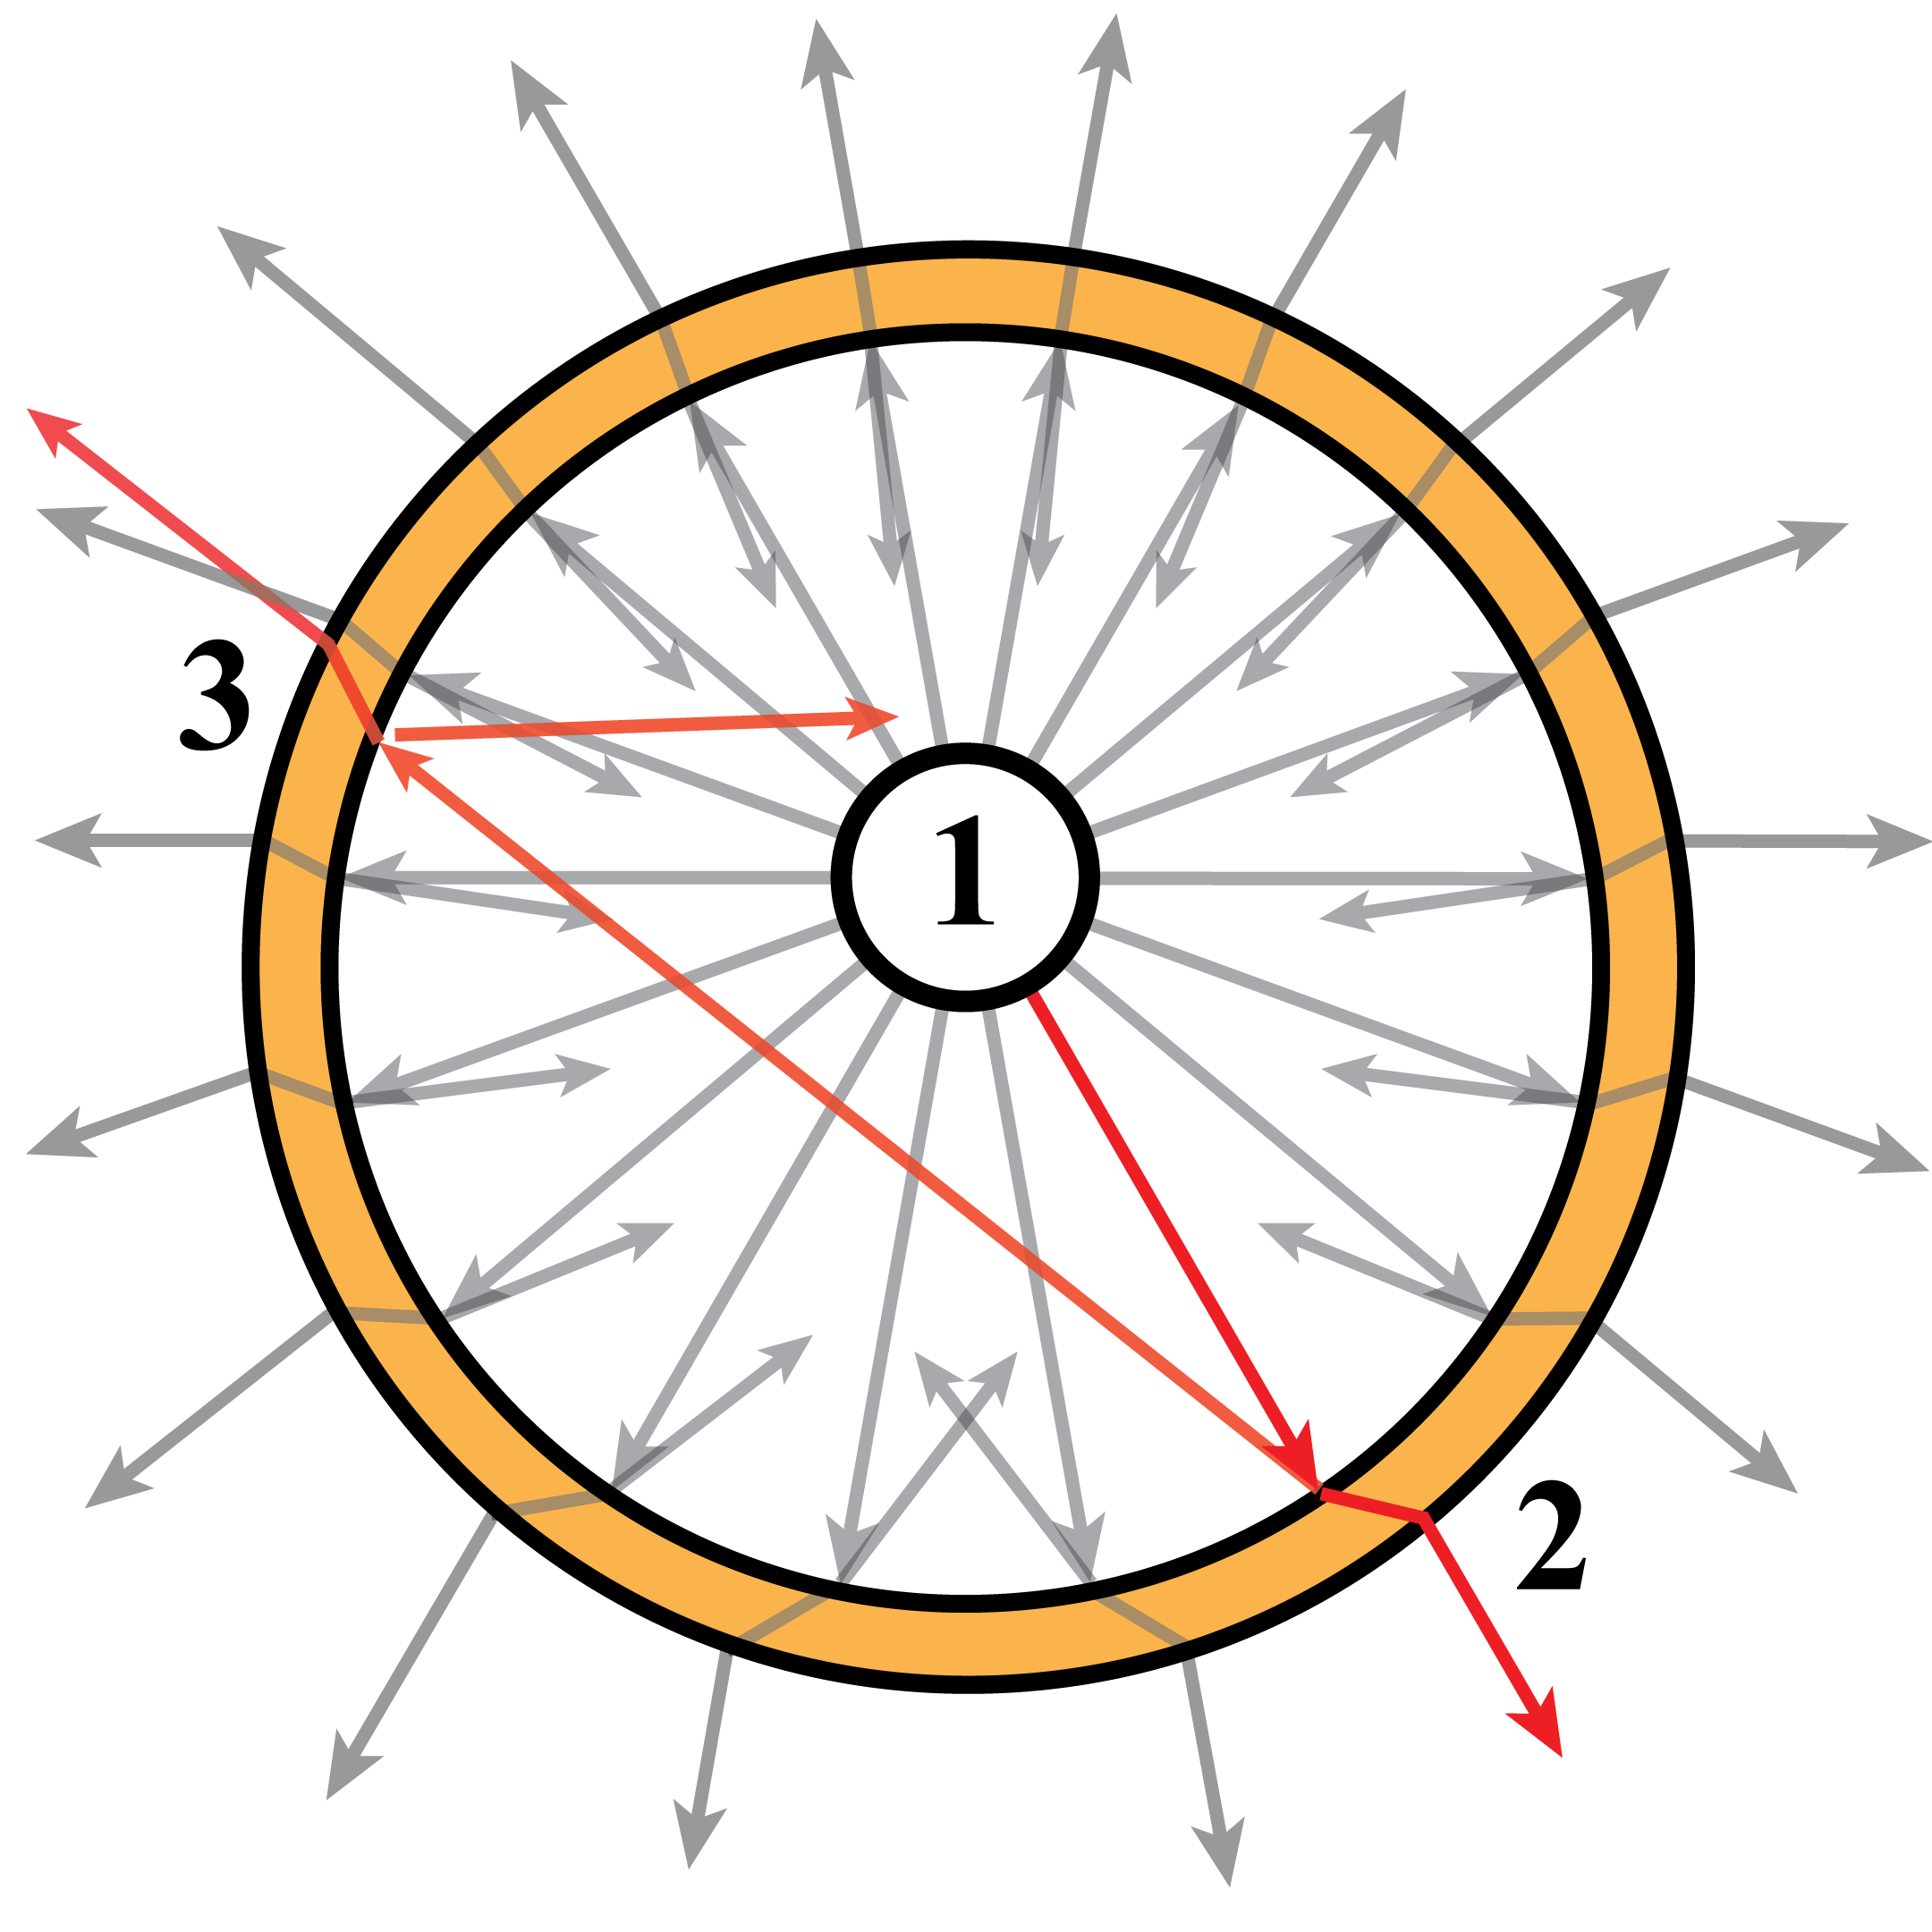
\includegraphics[width=\columnwidth]{future/informationProtection}
\caption[Proposed TR information protection system]{A proposed method of protecting a TR system from loss of information. The ``target'' of the TR process (1) is surrounded by a surface of semi-reflective material. This surface reflects effectively "splits" the outgoing wave into several smaller pieces (2). The result is that a greater solid angle is preserved coming out of the antenna/reflector system in cases such as the one in Fig.~\ref{fig:outgo}}
\label{fig:infoProtection}
\end{figure}

We believe that this concept should be tested using simulation methods as a proof-of-concept. Should it work we propose moving forward with some sort of experimental demonstration of information preservation effects. Finally, a model should be created describing the effectiveness of the method. Particular attention should be paid to the size of the design - we expect this method to be difficult to miniturize.

\subsection{Timing Analysis}

\subsection{Rectenna Design}
